%%%%%%%%%%%%%%%%%%%%%%%%%%%%%%%%%%%%%%
%% Introduction
%%%%%%%%%%%%%%%%%%%%%%%%%%%%%%%%%%%%%%

\section{Introduction}
\label{intro}

% One definition of form-finding
Tacos are a typical street food from Mexico.
Traditionally, there are three ingredients to tacos: tortillas, meat, and salsa \cite{lewis_computationalformfinding_2010, bletzinger_fiftyyears_2011}.

\subsection{Why do we care?}

We care about tacos because tacos are delicious.
We describe current approaches to make tacos in Section \ref{relatedwork}.

\subsection{Limitations of taco-making}
\label{limitations}

Current methods to make tacos face challenges and have limitations.

\subsubsection{Salsa is never right}
\label{salsa}

Taco lovers have to ask their neighbors if salsa is too spicy or not.
This is subjective and leads people to have their tongues hurt.
        
\subsubsection{Tortillas are cold}
\label{tortillas}

Taco makers forget to heat tortillas. Not crunchy, not good.

\begin{figure*}[t]
    \hspace{-2.0cm}
        \centering
        \begin{subfigure}[b]{0.37\textwidth}
            \centering
            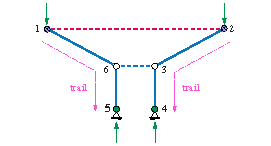
\includegraphics[width=\textwidth]{figures/tree_2d.pdf}
            \caption{Mexican cart}
            \label{fig:tree_2d}
        \end{subfigure}
        \hspace{-1.0cm}
        \begin{subfigure}[b]{0.37\textwidth}
            \centering
            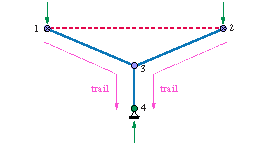
\includegraphics[width=\textwidth]{figures/tree_2d_wrong.pdf}
            \caption{Roma cart}
            \label{fig:tree_2d_wrong}
        \end{subfigure}
        \hspace{-1.0cm}
        \begin{subfigure}[b]{0.37\textwidth}
            \centering
            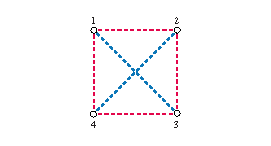
\includegraphics[width=\textwidth]{figures/square_tensegrity_wrong.pdf}
            \caption{Canasta vendor}
            \label{fig:self_stressed_wrong}
        \end{subfigure}
        \hspace{-2.0cm}
    
    \caption{Diagrams that correspond to three different taco-vending cart systems.}
    \label{fig:diagrams}
\end{figure*}

\subsection{Contributions}

We concretely describe our contributions.
\begin{enumerate}
    \itemsep 0em
    \item An automatic data-driven approach to calibrate salsa spiciness level.
    \item We add hot butter to the tortillas to keep them warm, oily, and delicious for longer.
  \end{enumerate}

\begin{table}[!b]
    \centering
    \begin{tabular}{@{}cll@{}}
    \toprule
    
    Type &
    Target &
    Constraint function \\
    
    \addlinespace[0.25em]
    \midrule
    \addlinespace[0.5em]
    
    Spiciness&
    Taco temperature, $\bar{\nodeposition_i}$&
    $\constraint_1( \equilibriumattributes(\optimizationvariables)) = \norm{\nodeposition_i - \bar{\nodeposition}_i}$\\
    
    \addlinespace[0.25em]
    \cmidrule(lr){1-3}
    \addlinespace[0.25em]

    \multirow{2}{*}[-6pt]{Heat}&
    Tortilla force, $\bar{\edgeforce}_{i, j}^{\text{t}}$&
    $\constraint_4(\equilibriumattributes(\optimizationvariables)) = \trailedgeforce_{i, j} - \bar{\edgeforce}_{i, j}^{\text{t}}$\\
    \addlinespace[0.5em]
    
    &
    Tortilla form, $\bar{\edgeloadpath}_{i, j}$&
    $\constraint_5(\equilibriumattributes(\optimizationvariables)) = \edgeforce_{i, j}\edgelength_{i, j} - \bar{\edgeloadpath}_{i, j}$\\
    \addlinespace[0.5em]
    
    \bottomrule
\end{tabular}
    \caption{Constraint functions supported by the our taco-making framework.}
    \label{constraints_table}
\end{table}

\subsection{Outline}
\label{outline}

This paper is organized in five sections: we survey the literature and compare our approach to existing taco-making methods in Section \ref{relatedwork}, we present our novel taco preparation approach in Section \ref{method}.
We carry out several experiments to numerically validate the proposed method in Section \ref{results}.
The paper concludes in Section \ref{conclusion} with a discussion of our experimental findings, the limitations of our approach and future research directions.